

\section{The Sinusoidal Distribution}
First we introduce the ``Standard" \sindist{} family as follows:

Random variable $Z$ is said to follow a Standard \sindist{} when it is distributed according to the density:
\begin{equation}
    \boxed{\psi(z; s,k) \equiv \frac{\varsigma(z; s,k)}{A(s,k)} = \frac{1}{A(s,k)} \sin^k(\pi z^s); \quad z \in [0,1]}
\end{equation}
where the parameters are $s \ge 0, k \ge 0$, the kernel is notated as $\varsigma(z; s,k) := \sin^k(\pi z^s)$, and $A(s,k) := \int_0^1 \sin^k(\pi t^s) \d t$ is the normalizing constant, i.e. the complete integral of the kernel over $[0,1]$. The notation for the distribution is $Z \sim \Sinu(s,k)$, and naturally, its CDF is given by:
\begin{equation}
    \Psi(z; s,k) = \int_0^z \psi(t; s,k) \d t \equiv \frac{A_z(s,k)}{A(s,k)}; \quad z\in[0,1]
\end{equation}
where $A_z(s,k)$ denotes the incomplete integral of the kernel.

We now introduce 2 extensions. Firstly, the location scale extension is defined as follows: random variable $X$ follows a location-scale \sindist{} family, notated $X \sim \Sinu(a,d,s,k)$ with parameters $a \in \RR, d \ge 0, s \ge 0, k\ge 0$, when $X$ has density:
\begin{equation}
    \psi(x; a,d,s,k) = {\frac 1 d} \psi \left( \frac{x-a}{d}; s,k \right);  \quad x \in [a, a+d]
\end{equation}

Next, we introduce a ``flipped extension" (for the reason described in \autoref{subsec:shape}, \autoref{item:flippedsinureason}) to the \sindist: random variable $X$ follows a flipped location-scale \sindist{} family, notated $X' \sim \Sinu'(a,d,s,k)$, when $X' :\overset{d}{=} a+d - X$ where $X \sim \Sinu(a,d,s,k)$. Conceivably, $X'$ has density
\begin{equation}
    \psi'(x; a,d,s,k) = {\frac 1 d} \psi \left( \frac{a+d-x}{d}; s,k \right)
\end{equation}

\begin{comment}
\subsubsection*{Multivariate Extension}
We provide multivariate extension notions of only the standard \sindist{}, i.e. location scale extensions of the multivariate extensions is left implicit.

A: Defined independently using individual (s,k)'s: $\vec Z_{m \times 1} \sim \psi_m( \vec s_{m \times 1}, \vec k_{m \times 1})$:
\[\psi_m (\vec z; \vec s, \vec k) = \prod_{j=1}^m \psi(z_j; s_j,k_j)\]
This makes it equivalent to the joint density of $m$ independent Standard Sinusoidal random variables.

B: Defined through a common $(s,k)$ pair via vector generalization
\[ \psi_m (\vec z; \mat D, s, k) = \psi ( \vec z^\intercal \mat D^{-1} \vec z ; s, k) \]
Unsure of the structure of D, what kind of correlation structure D will provide, whether the defined density will be normalized, how s and k will influence its shape here, etc.

C: Defined through the Archimedean copula.
\end{comment}

\autoref{fig:shapeplots} illustrates the PDFs, CDFs, Hazard functions and DQFs (Density-Quantile Functions, as described in \cite{staudte2017dqf}) of some Standard \sindist s.

%\begin{landscape}
   \begin{figure}
        \begin{subfigure}{0.49\linewidth}
            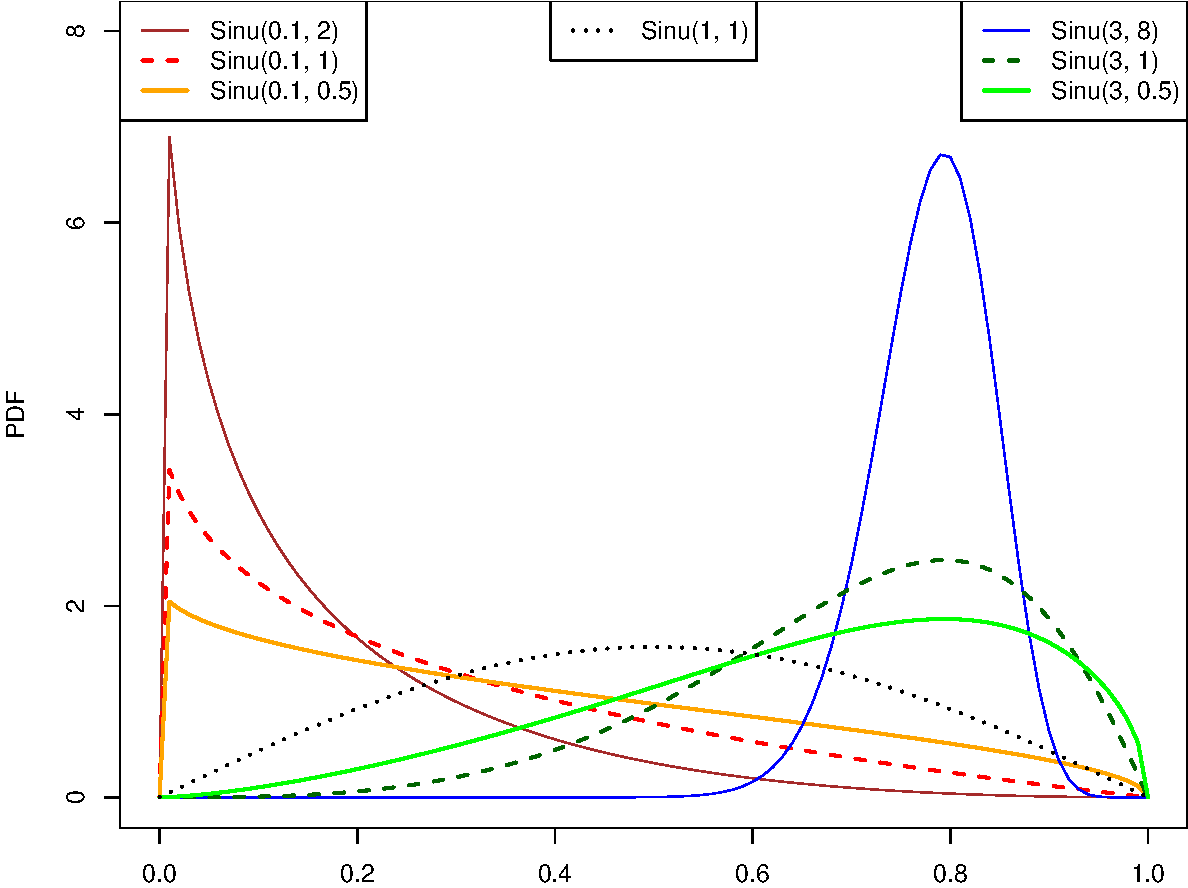
\includegraphics[width=\linewidth]{fig/2-pdf}
            \caption{PDFs}
        \end{subfigure}
        \begin{subfigure}{0.49\linewidth}
            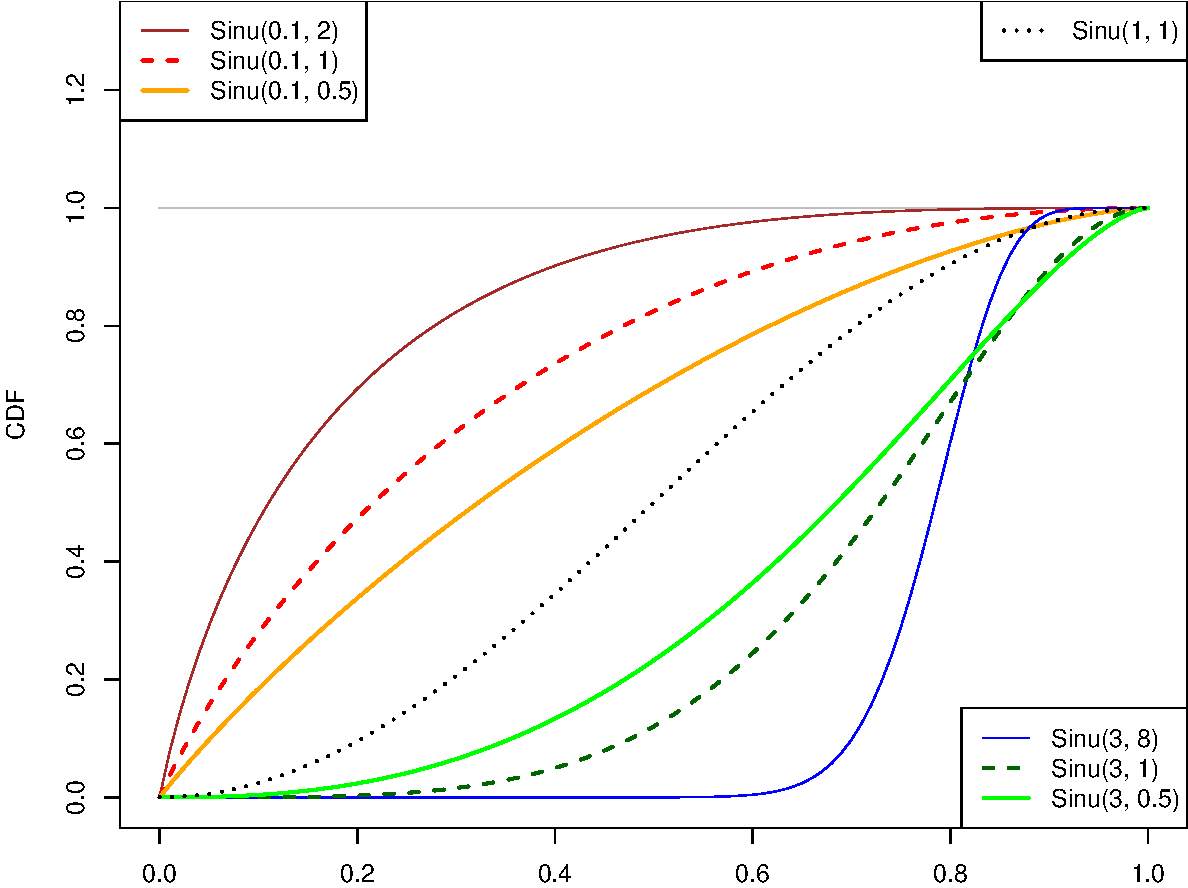
\includegraphics[width=\linewidth]{fig/2-cdf}
            \caption{CDFs}
        \end{subfigure}
        \begin{subfigure}{0.49\linewidth}
            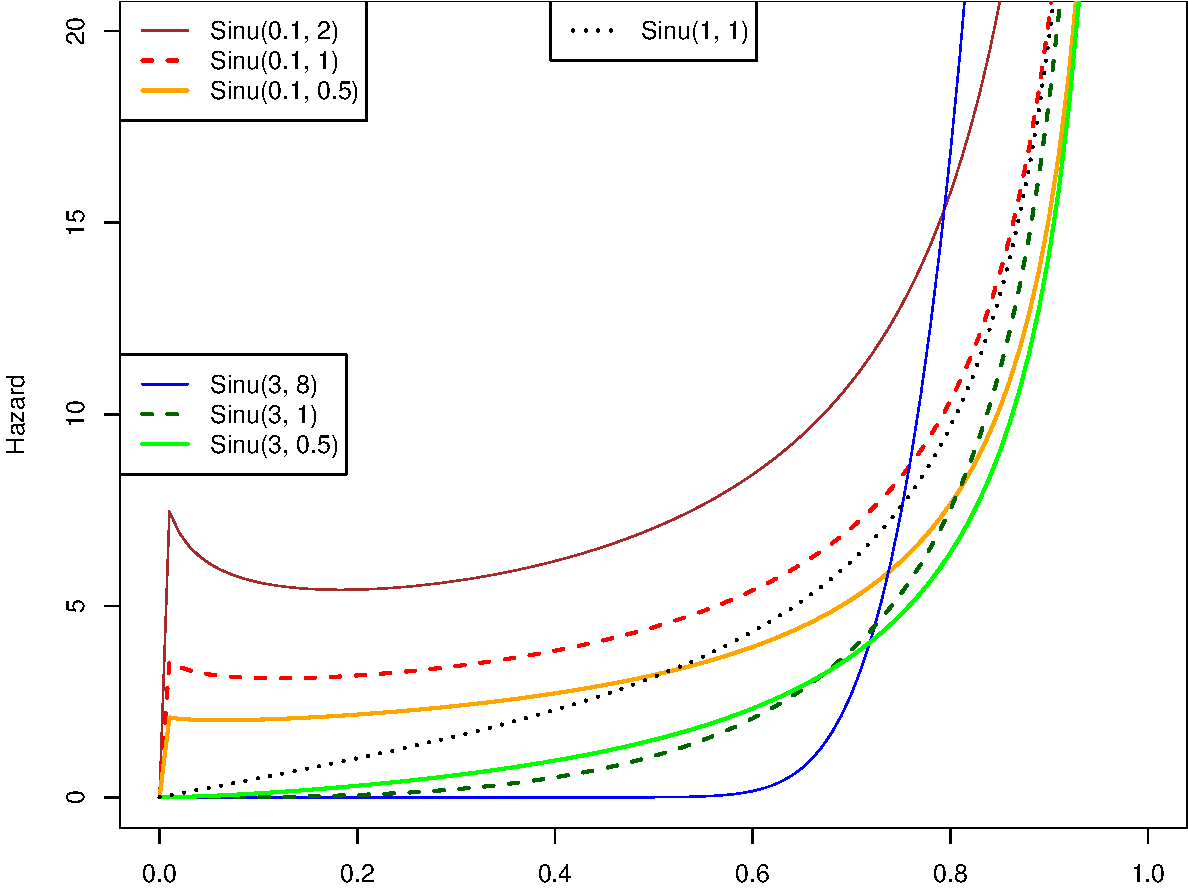
\includegraphics[width=\linewidth]{fig/2-hf}
            \caption{Hazard Functions}
        \end{subfigure}
        \begin{subfigure}{0.49\linewidth}
            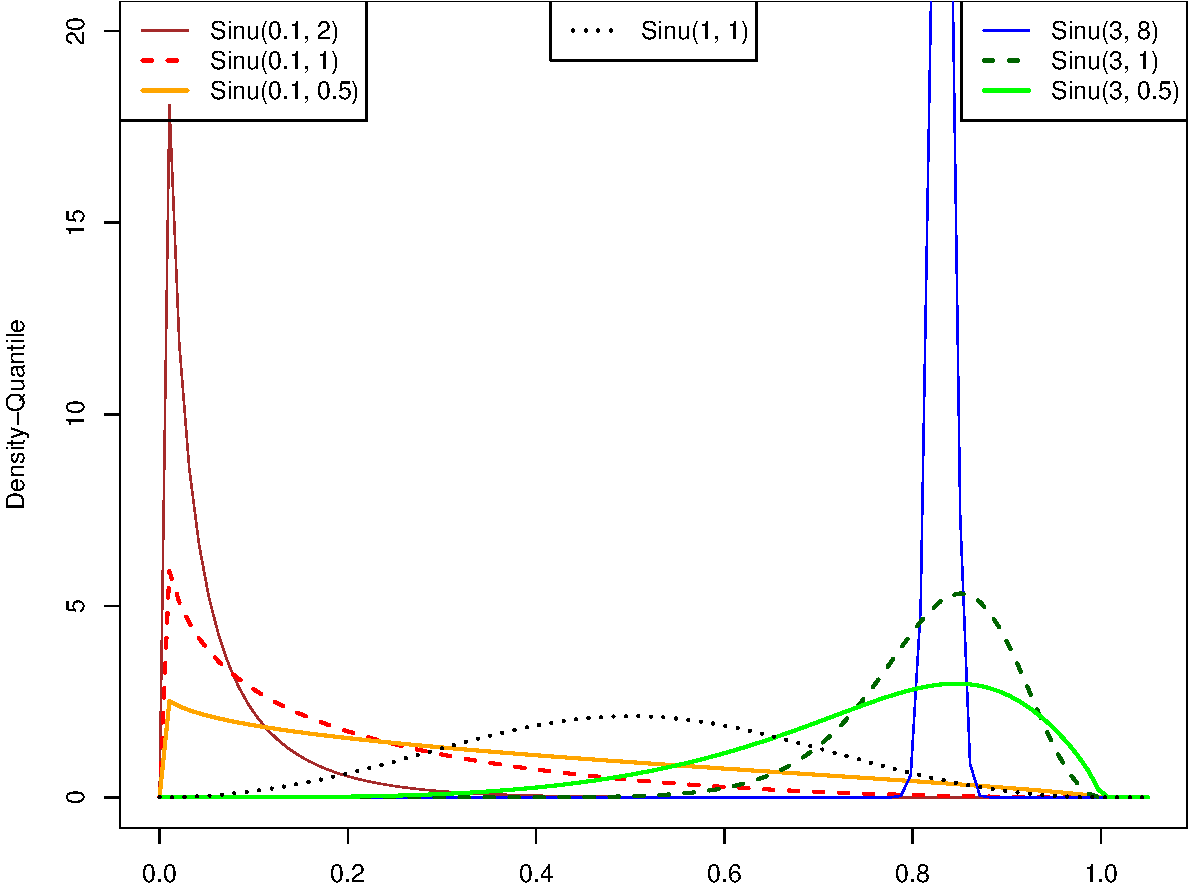
\includegraphics[width=\linewidth]{fig/2-dqf}
            \caption{DQFs}
        \end{subfigure}
        \caption{Shape plots of different \sindist s}\label{fig:shapeplots}
    \end{figure}
%\end{landscape}

\subsection{Shape Properties}\label{subsec:shape}
Some shape properties of the \sindist{} are discussed below:
\begin{enumerate}
    \item Support: $[a, a+d]$. $a$ is the location and $d$ is the scale parameter. Alternative parametrization with $b=a+d$ may be considered.
    \item $s$ affects skewness of the \sindist{} as follows:
    \begin{enumerate}
        \item $0 < s <1$: left-leaning (positively/right skewed)
        \item $s=1$: symmetric
        \item $s>1$: right-leaning (negatively/left skewed)
    \end{enumerate}.
    The alternative parametrization $s' = \ln s$ calibrates the parameter choice $s=0$ to the symmetric family, and on either side of it keeps oppositely signed skewness families.
    \item The choice $a=-\frac d 2$, $s=1$ gives the special symmetric around 0 $\Sinu(-\frac d 2, d, 1, k)$ family, supported on the interval $[-\frac d 2, \frac d 2]$.
    \item $s$ (or any transformation of it) does not affect the shape of the distribution symmetrically around the point $s=1$; i.e. $\nexists s'{<1}: \Sinu(s', k) \overset{d}{=} 1-\Sinu(s,k) \quad \forall s{>}1$. It is for this reason that we introduced the notion of a flipped \sindist{}.\label{item:flippedsinureason}
    \item $k$ affects kurtosis non-monotonically. See \autoref{fig:skassoc}.
    \item $s, k$ jointly affect both the skewness and the kurtosis. See \autoref{fig:skassoc}.
   \begin{figure}
        \begin{subfigure}{0.48\linewidth}
            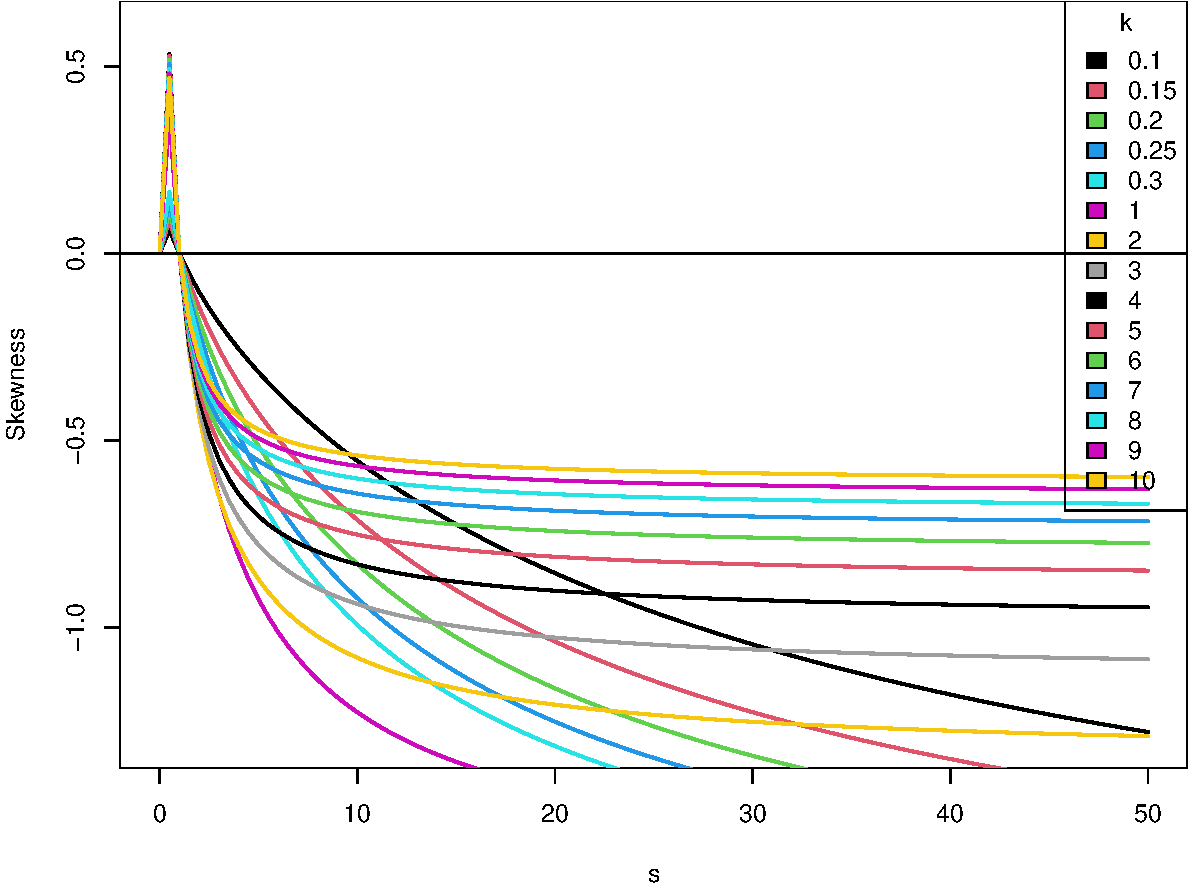
\includegraphics[width=\linewidth]{fig/2-skewvss}
            \caption{Skewness vs. $s$}
        \end{subfigure}
        \begin{subfigure}{0.48\linewidth}
            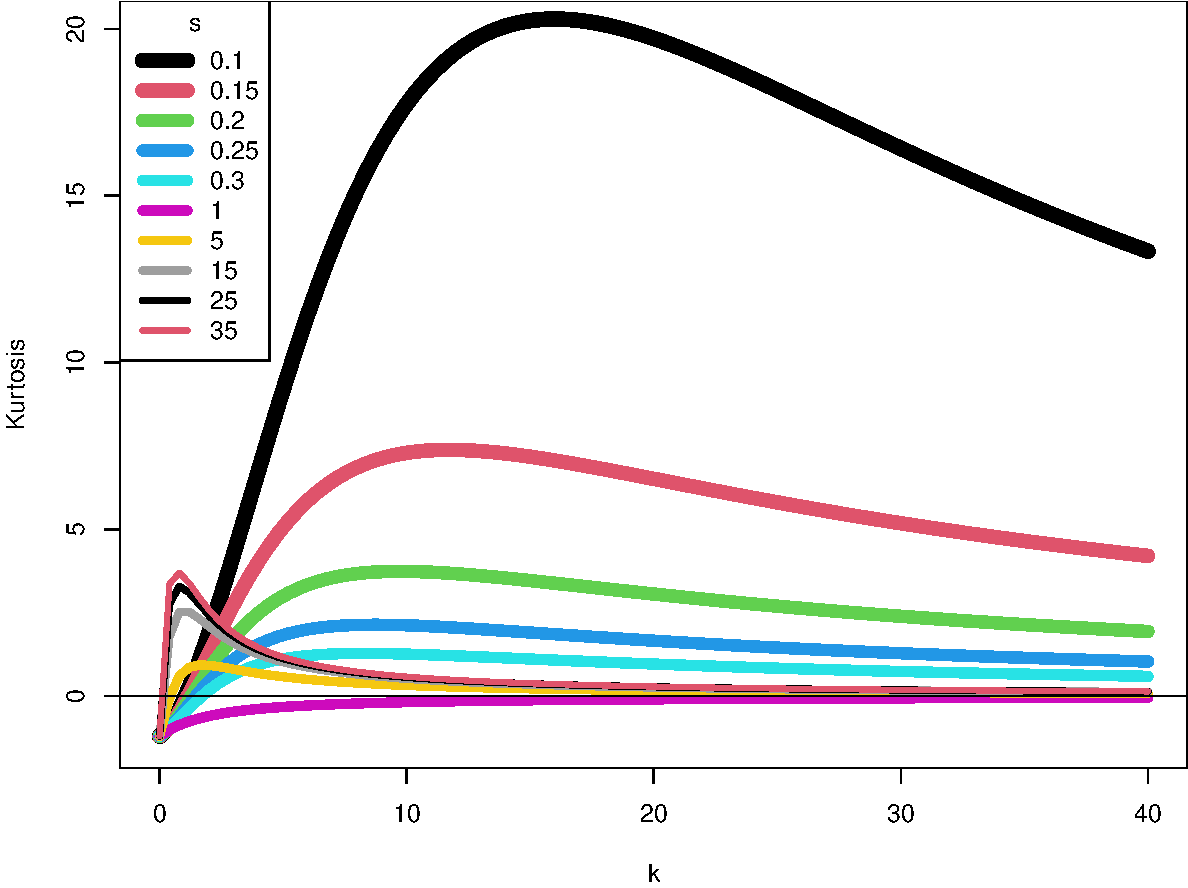
\includegraphics[width=\linewidth]{fig/2-kurtvsk}
            \caption{Kurtosis vs. $k$}
        \end{subfigure}
        \caption{$s$, $k$ jointly affect skewness \& kurtosis}\label{fig:skassoc}
    \end{figure}
    \item A $\Unif(a,a+d)$ density results from the \sindist{} density when k=0 or s=0.
    \item Degenerate at $a$ for $d=0$
    \item $\Sinu(-\frac{d}{2}, d, 1, k) \xrightarrow[d=\pi \sqrt k]{k \to \infty} \N(0,1)$. See \autoref{thm:normality}.
    \item The mode of $\Sinu(s,k)$ is $2^{-1/s}$ and the modal density is $1/A(s,k)$. See \autoref{thm:mode}.
\end{enumerate}


\section{Preliminary Mathematical Properties}
Proofs to theorems mentioned are provided in the Appendix \autoref{subsec:app-prelim_math}.
\begin{comment}
\subsection*{Programmatic Notation}
We follow these conventions of nomenclature, in both the report and the code as far as possible, to quickly understand the domain of variables, and in some ways also their interpretation.
\begin{enumerate}
    \item $x \in [a, a+d]$
    \item $z :\equiv\frac{x-a}{d} \in [0,1]$
    \item $u :\equiv z^s\in [0,1]$ also.
    \item $\theta :\equiv \pi u \equiv \pi z^s \in [0,\pi]$
    \item $\omega := \theta - \frac{\pi}{2} \equiv \pi z^s - \frac{\pi}{2} \in [-\frac{\pi}{2}, \frac{\pi}{2}]$
    \item $r = \pm 1$
\end{enumerate}
\end{comment}

\subsection{Physical Interpretation}
Similar to \cite{gilbert1893moon} -- which imagines intensity (interpreted as probability density) of crater activity on a circular planet as proportional to Gilbert's Sine density $\sin\theta$ -- the Standard \sindist{} $\Sinu(s,k)$ can also be physically interpreted as the intensity of crater activity on a (possibly non-circular) planetary surface given by the radial curve:
\begin{equation}
    r(z) = r_0 \exp\left(\int_0^{\pi z^s} \tan(t - \sin^{-1}\sin^k t) \d t\right)
\end{equation}
where the curve $r(z)$ is parametrized by $z \in [0,1]$ such that $\theta=\pi z^s$ is the angle the location $r(z)$ subtends at the origin, and $r_0$ is the initial radius at $z=0$. Details are furnished in \autoref{rmk:planet}.

\begin{comment}
\subsection{Transformation}
\begin{thm}[Expression as a morphed arcsin Beta distribution] \label{thm:transform}
    $Y \sim \Beta(\frac{k+1}{2}, \frac{1}{2})$ and $R \sim \Ber (\frac 1 2)$, then
    \[Z = \left[ R \sin^{-1} \sqrt Y + (1-R) (\pi - \sin^{-1} \sqrt Y) \right]^\frac{1}{s}\]
    follows a $\Sinu(s,k)$ distribution.
\end{thm}
\end{comment}



\begin{thm}[Joint density expression]\label{thm:jtdens}
    For $X_1\dots X_n \iidsim \Sinu(a,d,s,k)$, their joint density can be expressed as:
    \begin{equation}
        f(x_1\dots x_n) = \frac{1}{A^n(s,k) 2^{nk} d^n } \left( \sum_{r_1=\pm1}\cdots \sum_{r_n = \pm 1} \left[\prod_{j=1}^n r_j\right] \cdot \exp\left[\sum_{j=0}^n \i \pi r_j \left(\frac{x_j -a}{d}\right)^s\right]  \right)^k
    \end{equation}
\end{thm}

\subsection{Concentration Inequalities}
\begin{thm}[\sindist{} is sub-Gaussian]
    $X \sim \Sinu (a,d,s,k)$ is sub-Gaussian with parameter $\frac{d^2}{4}$.
\end{thm}
\begin{proof}
    $\because a \le X \le a+d \quad\text{a.s.}$, $\therefore \E \left[ \e^{\lambda (X - \E X)} \right] \le \exp \left( -\frac{\lambda d^2}{8} \right)$ by Hoeffding's lemma.

    Note that because it is sub-Gaussian, it is also sub-Exponential.
\end{proof}


\subsection{Normalizing constant for the symmetric case}
\begin{thm}[Normalizing constant, symmetric case]\label{thm:norm_sym}
    \begin{align}
        A(1,k) \equiv \int_0^1 \sin^k(\pi t) \d t &= \frac{2^k}{\pi} \frac{\Gamma^2\left( \frac{k+1}{2} \right)}{\Gamma\left( k+1\right)} \label{eq:area1}\\
        &= \frac{1}{\sqrt \pi} \frac{\Gamma\left(\frac{k+1}{2}\right)}{\Gamma\left(\frac{k}{2} + 1\right)} \label{eq:area2}
    \end{align}
\end{thm}


\subsection{Incomplete integral of the kernel for the Symmetric case}
\begin{thm}[Incomplete integral of the kernel for the symmetric case] \label{thm:cdf_sym}
    When $k\in \ZZ^+$, $s=1$, we have --
    \begin{align}
        \int_0^z \sin^k\pi t \, dt &=
        \frac{1}{2^{2n}} {2n \choose n} z + \frac{(-1)^n}{\pi 2^{2n-1}}\sum_{k=0}^{n-1} (-1)^k {2n \choose k} \frac{\sin 2(n-k)\pi z}{2(n-k)} && [\text{$k$ even}]\\
        &= \frac{1}{\pi 2^{2n}}(-1)^n \sum_{k=0}^n (-1)^k {2n+1 \choose k} \frac{1 - \cos (2n+1-2k)\pi z}{2n+1-2k}  &&  [\text{$k$ odd}]
    \end{align}
\end{thm}


\subsection{Limiting to Normality}
\begin{thm}\label{thm:normality}
    For the symmetric about 0 \sindist{} $\Sinu\left(-\frac{d}{2}, d, 1, k\right)$, i.e. with $a = -\frac{d}{2}$ and $s=1$, setting $d \equiv d(k)= \pi \sqrt k$ and letting $k \uparrow \infty$, we have:
    \[ \psi_k(x) \to \phi(x)\]
    where $\phi(x)$ is the PDF of a Standard Normal distribution.
\end{thm}



\section{Properties involving the Generalized Hypergeometric Function}
For this section, we define Generalized Hypergeometric Function (GHGF) $\Fhyp_q^p$, parametrized by $a_1, \dots, a_p$ and $b_1, \dots, b_p$, calculated at the argument $x$ as: 
\[\Fhyp_q^p \left(\begin{matrix} a_1 & \cdots & a_p \\ b_1 & \cdots & b_q\ \end{matrix} ; x \right) := \sum_{j=0}^\infty \frac{\poch{a_1}[j] \cdots \poch{a_p}[j]}{\poch{b_1}[j] \cdots \poch{b_q}[j]} \frac{x^j}{j!}\]
where $\poch x := x(x+1)\cdots(x+n-1)$ is the rising factorial / Pochhammer function.

Also define from hereon ${r \choose k} = \frac{\poch{r}[k]}{k!}$ as the generalized binomial coefficient.

Some additional notes are provided in \autoref{rmk:ghgf}. Proofs to the theorems mentioned are provided in \autoref{subsec:app-prop_ghgf}.

\subsection{Kernel}
\begin{thm}[Kernel expression via Binomial expansion of Euler form]\label{thm:kernelbin}
    \begin{equation}\label{eq:kernelbin}
        \varsigma(z; s,k) \equiv \sin^k (\pi z^s) =  \frac{1}{(2\i)^k} \sum_{j=0}^\infty (-1)^j {k \choose j}  \e^{\i (k-2j) \pi z^s}
    \end{equation}
\end{thm}

\begin{thm}[Kernel expression via Generalized Hypergeometric Function]\label{thm:kernelhgf}
    \begin{align}
        \varsigma(z; s,k) \equiv \sin^k (\pi z^s) &=  (\pi z^s)^k \left( \Fhyp^0_1 \left[ \begin{matrix} \cdot \\ \frac{3}{2} \end{matrix}; -\frac{\pi^2 u^2}{4}\right] \right)^k \label{eq:kernelghfreal}\\
        &= \Fhyp^1_0 \left[ \begin{matrix}k\\ \cdot\end{matrix};  -\exp(-2 \i \pi z^s) \right] \label{eq:kernelhgfcomplex}
    \end{align}
\end{thm}

\subsection{CF and MGF}
\begin{thm}[Characteristic Function and MGF of the Standard \sindist] \label{thm:cfmgf}
    For $Z \sim \Sinu(s,k)$, its CF is given as --
    \begin{equation}\label{eq:cf}
        \varphi_Z(t) = \frac{1}{A(s,k) (2\i)^k} \sum_{j=0}^{\infty} (-1)^j \binom{k}{j} \sum_{m=0}^{\infty} \frac{(\i t)^m}{(m+1)!} \Fhyp^1_1\left[ \begin{matrix}\frac{m+1}{s}\\ \frac{m+1}{s} + 1 \end{matrix};\, \i\pi(k-2j) \right]
    \end{equation}
    Additionally, the MGF is given as --
    \begin{equation}
        \upphi_Z(t) \equiv \varphi_Z(-it) = \frac{1}{A(s,k) (2\i)^k} \sum_{j=0}^{\infty} (-1)^j \binom{k}{j} \sum_{m=0}^{\infty} \frac{t^m}{(m+1)!} \Fhyp^1_1\left[ \begin{matrix}\frac{m+1}{s}\\ \frac{m+1}{s} + 1 \end{matrix};\, \i\pi(k-2j) \right]
    \end{equation}
\end{thm}

\subsection{Moments}
\begin{thm}[Moments of Standard \sindist]\label{thm:moments}
    For $Z \sim \Sinu(s,k)$, $\upmu_r(s,k) := \E [Z^r]$ is given by
    \begin{align}
        \upmu_r(s,k) &= \frac{1}{A(s,k) (2\i)^k (r+1)} \sum_{j=0}^{\infty} (-1)^j \binom{k}{j} \Fhyp^1_1 \left[ \begin{matrix}\frac{r+1}{s}\\ \frac{r+1}{s} + 1\end{matrix}; \, \i\pi(k-2j) \right]\\
        &= \frac{1}{A(s,k) (2\i)^k} \sum_{j=0}^\infty {k \choose j} (-1)^j \sum_{n=0}^{\infty} \frac{[\i (k-2j) \pi]^n}{n! (ns+r+1)}
    \end{align}
\end{thm}

\subsection{CDF}
\begin{thm}[CDF of the Standard \sindist]\label{thm:cdf}
    \begin{equation}
        \Psi(z; s,k) = \frac{1}{A(s,k) (2\i)^k} \sum_{j=0}^\infty (-1)^j {k \choose j} \sum_{n=0}^{\infty} \frac{[\i (k-2j) \pi]^n}{n! (ns+1)} z^{ns+1}
    \end{equation}
\end{thm}

\subsection{Normalizing constant}
\begin{thm}[Normalizing constant for the Standard \sindist{}]
    \[A(s,k) = \frac{1}{(2\i)^k} \sum_{j=0}^\infty (-1)^j {k \choose j} \sum_{n=0}^{\infty} \frac{[\i (k-2j) \pi]^n}{n! (ns+1)} \]
\end{thm}


